\documentclass{article}
\usepackage[utf8]{inputenc}
\usepackage{amsmath}
\usepackage{graphicx}
\usepackage{BeginnerStyleFile}
\graphicspath{ {images/} }

\title{Reading Summary Appendix A, B}
\author{Evan Hughes}
\date{January 2023}

\begin{document}

\maketitle
\section{Appendix A$\colon$ Logic and Proof}
\subsection*{Propositions}
A \textbf{proposition} is a declarative statement that can be either true or false.

EX$\colon$ 2 is a positive integer
\subsection*{Compound Statements}
A \textbf{compound statement} is when two or more statements are combined using words like "or" and "and."

$P$ and $Q$ is true when both $P$ and $Q$ are true, otherwise it is false.

$P$ or $Q$ is true when one or both are true and false when both are false.
\subsection*{Negation}
\textbf{Negation}($\lnot$) changes the meaning of a proposition by inverting it.
Changing its outcome from false to true and vice versa.

\subsection*{Quantifiers}
Universal quantifiers ($\forall$) are used to state that a statement is true for all values of a variable.
EX$\colon$ For all $x$, $x^2$ is a positive integer.


Existential quantifiers ($\exists$) are used to state that a statement is true for at least one value of a variable.
EX$\colon$ There exists a positive integer $x$ such that $x^2$ is a perfect square.


The negation of a statement with a universal quantifier
is a statement with an existential quantifier. 

\subsection*{Conditional Statements}
A \textbf{conditional statement} is a statement is a \emph{if-then} statement.

EX$\colon$ If $x$ is a positive integer, then $x^2$ is a positive integer.


Conditional statements are written symbolically as $Q \implies P$ 
\
$P \implies Q$ is a true statement when both P and Q are
true and false when P is true and Q is false. 
The contrapositive of the conditional statement $P \implies Q$ is the statement $\lnot Q \implies \lnot P$. 
\subsection*{Proofs}

There are 3 main types of proofs:
\begin{itemize}
    \item Direct Proof
    \item Contrapositive Proof
    \item Proof by Contradiction
\end{itemize}

\subsection*{Direct Proof}
A \textbf{direct proof} is a proof that shows that a statement is true by showing that each of its premises is true.
This method relies on the rule of logic called 
\textbf{modus ponens$\colon$} If $R$ is a true statement and $R \implies S $ is a true conditional
statement, then $S$ is a true statement.


\textbf{Example$\colon$} To prove the theorem $ P \implies Q$ by the direct
method, you find a series of statements $P_1$, $P_2$,\ldots, $P_n$ 
and the verify that each of the implications $P_n\implies P_{n+1}$ is true.
Then
the assumption that $P$ is true and repeated use of \textbf{modus ponens} show that $Q$ is true.

\subsection*{Contrapositive Proof}
A \textbf{contrapositive proof} is a proof that shows that a statement is true by showing that the contrapositive of the statement is true.
\begin{figure}[h]
    \centering
    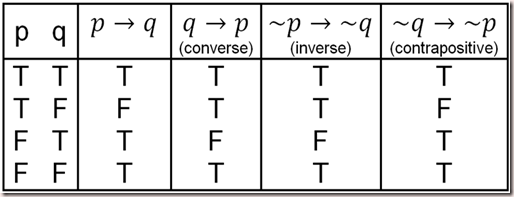
\includegraphics[scale=0.5]{contrapositive.png}
    \caption{Contrapositive Truth Table}\label{fig:contrapositive truth table}
\end{figure}
\subsection*{Proof by Contradiction}
A \textbf{proof by contradiction} is a proof that shows that a statement is true by showing that the negation of the statement is false.

To prove a multi conditional statement you must prove all parts of it.

\newpage
\section{Appendix B$\colon$ Sets and Functions}
\subsection*{Sets}
A \textbf{set} is a collection of objects.

\end{document}
